\documentclass{scrartcl}
%\documentclass[11 pt, a4paper,twosided,titlepage]{scrartcl}
% Defines citation style
\usepackage [super , square , sort&compress ]{natbib}

%\usepackage[ngerman]{babel} 
\usepackage[utf8]{inputenc}
\usepackage[T1]{fontenc}
\usepackage{lmodern}

% math
\usepackage{amsmath}
\usepackage{amssymb}

\usepackage{graphicx}

\usepackage{booktabs}
% set special behaviour for hyperlinks in pdfs
\usepackage[breaklinks=true]{hyperref}

\usepackage{listings}

\usepackage{blindtext}

\usepackage{xcolor}

\usepackage{siunitx}
\sisetup{exponent-product = \cdot, output-product = \cdot}


\begin{document}
	
\title{Our first paper}
\author{Julian Huber}
\date{Winter 2022}
\maketitle

\abstract{\blindtext}

% This is not common in articles
\tableofcontents


\section{Commands in Latex}

This is a \emph{nice} article. \\ In which we force a new line.

% \test

\section{Markups in Latex}


It      does        not     matter      how     many    blanks   we     use. 	

This \textit{is} a \emph{nice} \textbf{article}.


\section{Modular Documents}

This is text from the sub article!


\section{Environments in Latex}


\subsection{Lists}

\begin{itemize}
	\item Frist
	\item Second
	\item Third
\end{itemize}

Anführen sollte man auch noch:
\begin{enumerate}
	\item Manche mögen die Grünen am liebsten,
	\item manche die Gelben.
	\item Ich mag am liebsten die Roten.
	\begin{enumerate}
		\item Sie glühen richtig rot,
		\item und ihr Himbeergeschmack fährt wie Napalm über
		die Geschmacksknospen.
	\end{enumerate}
\end{enumerate}

\begin{description}
	\item[Das Schlagwort] steht am Anfang einer Zeile und wird
	hervorgehoben, während der zugehörige
	\item[Text] dahinter in normaler Schrift erscheint.
\end{description}


\section{Headings}


% We can define a shorter title for the TOC
\subsection[Short Title]{This a a very long title line}

% We can force the TOC to ignore headings
\subsection*{This won't be shown and does not get a number}


\section{Packages}


We can use \textcolor{orange}{colored text} now.



\subsection{Figures}

Figure~\ref{fig:AbleitungHyperbel} describes a hyperbola.

\begin{figure}[h]
	\centering
	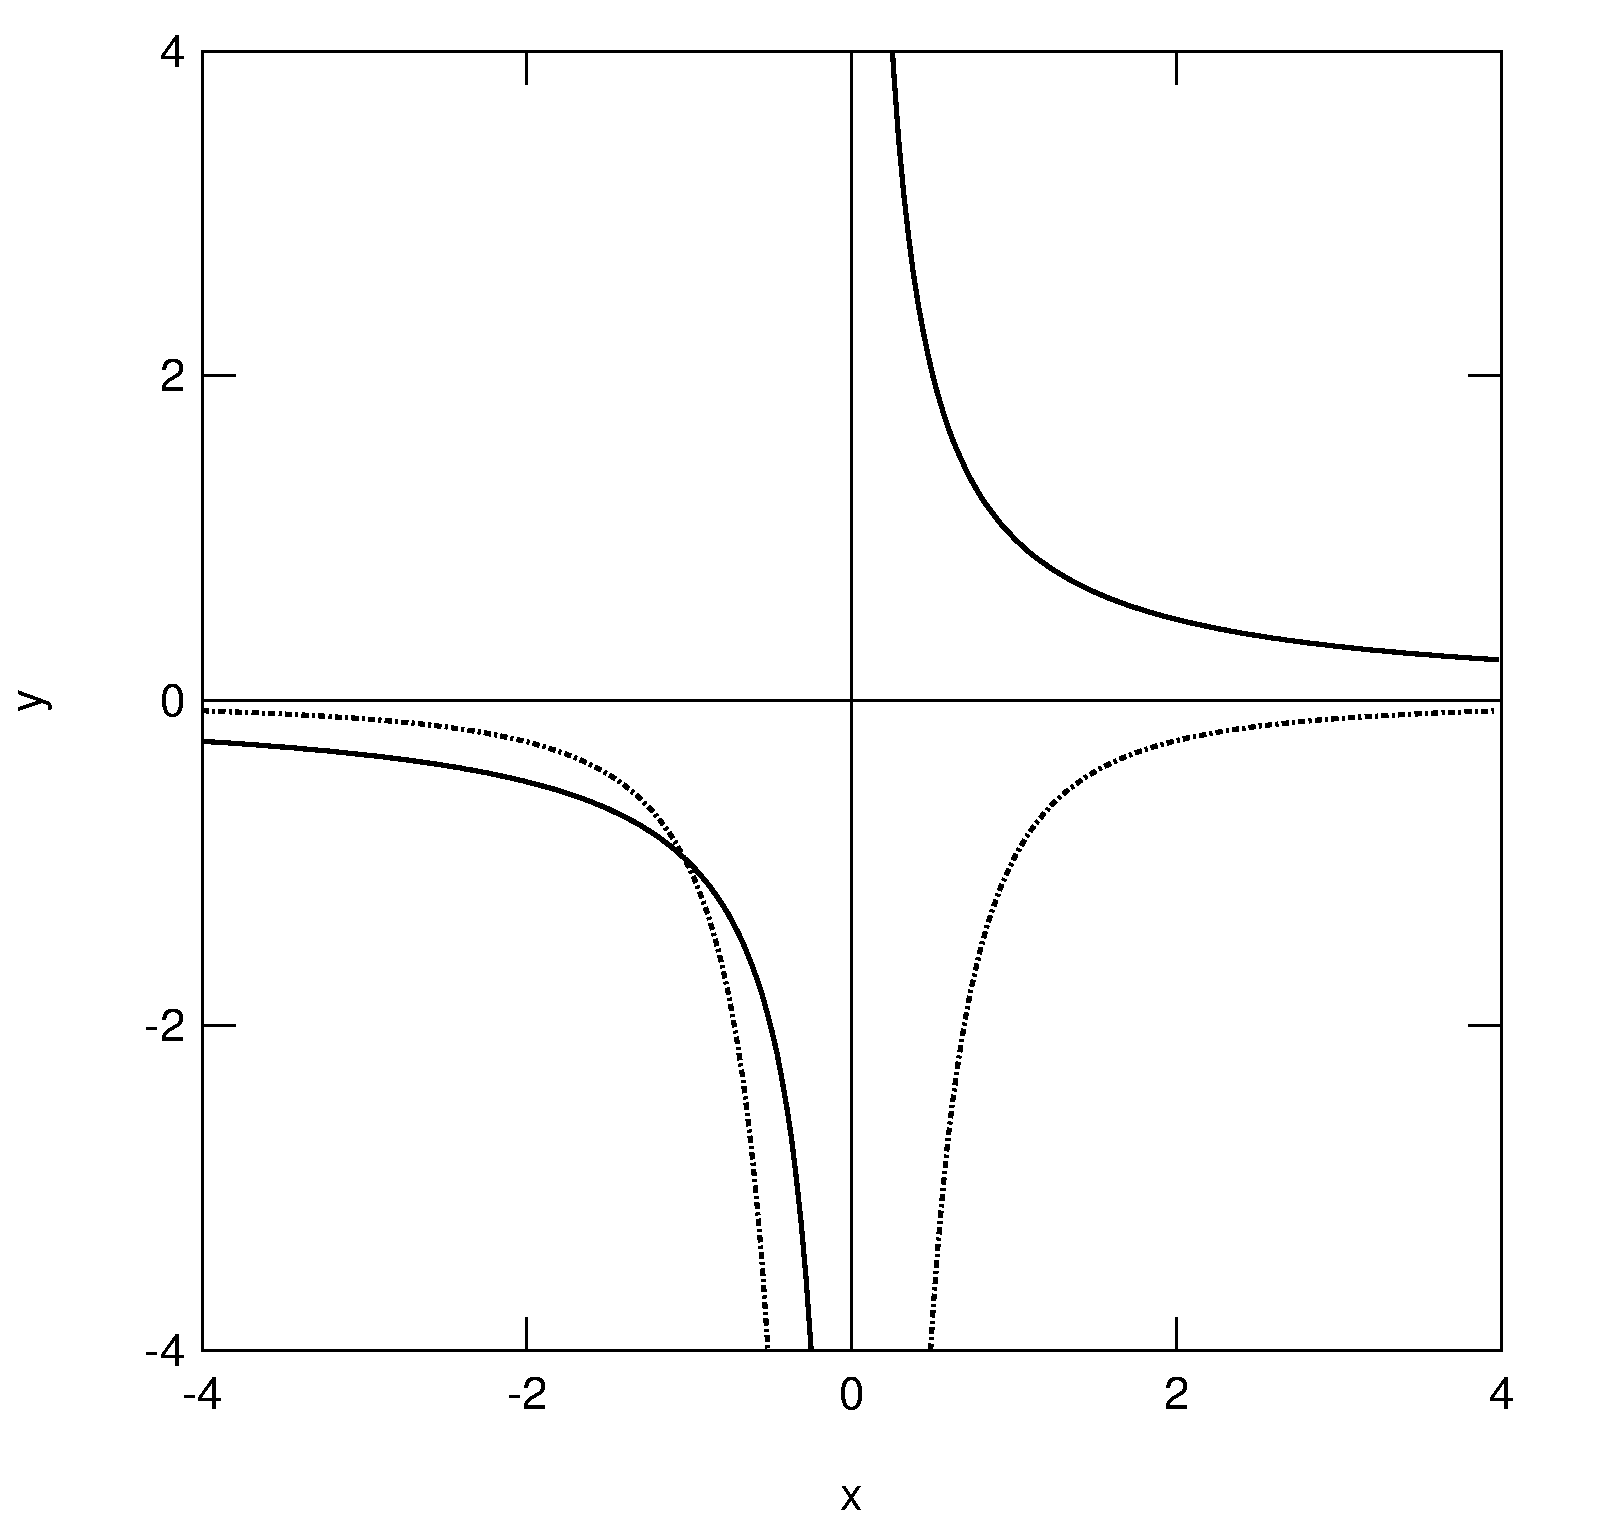
\includegraphics[width=0.5\textwidth]{HyperbelAbleitung-eps-converted-to.pdf}
	\label{fig:AbleitungHyperbel}
	\caption[Hyperbel und Ableitung.]{Die durchgezogene Linie ist eine Hyperbel, die strich-punktierte  Linie ist die Ableitung einer Hyperbel.}
\end{figure}

\subsection{Tables}

\begin{table}[ht]
	\begin{center}
		\caption{The table caption comes above the table}
		\begin{tabular}{l|cr}
			\toprule
			Spalte 1 & Spalte 2 & Spalte 3\\
			\midrule
			AA & AB & AC\\
			BA & BB & BC\\
			CA & CB & CC\\
			\bottomrule
		\end{tabular}
	\end{center}
\end{table}

\subsection{Math Mode}

\subsubsection{Equation}
\begin{equation}
	x=2
	\label{eq:x_is_two}
\end{equation}

\subsubsection{Listings}
\begin{lstlisting}[caption = Wege in den Mathematikmodus, label = ReininMathe]
	Mittels \emph{equation}-Umgebung:
	\begin{equation}
		a^2+b^2=c^2
		\label{Pythagoras}
	\end{equation}
	Mittels einfachen Dollarklammern: $a^2+b^2=c^2$\\
	Mittels doppelten Dollarklammern: $$a^2+b^2=c^2$$
\end{lstlisting}


	\begin{equation}
	a^2+b^2=c^2
	\label{Pythagoras}
\end{equation}
Mittels einfachen Dollarklammern: $a^2+b^2=c^2$\\
Mittels doppelten Dollarklammern: $$a^2+b^2=c^2$$

\subsubsection{Examples}

$$x = 5\cdot 2^{20} \cdot \frac{\Omega}{\omega}$$
$$\sum_{i=0}^{n}(X_i)$$
$$1^{2^3}$$
$$0= \sin{x} + \ln{x}$$
$$ \vec{V} = \hat{u}$$

\subsubsection{Physical  Quantities}

$$l= 10 \text{m}$$


$$k=\SI{1.38e-23}{\joule \per\kelvin}$$

$$h=\SI{6.626e-34}{\joule \second}$$

$$\varepsilon_0=\SI[per-mode=fraction]{8.854e-12}{\ampere \second \per\volt \per\meter}$$

$$\SI{8000}{\kilo\gram\of{Metall} \per\hour}$$

\section{Citations}
This is a \emph{nice} article \cite{lemola2007maternal}.


\bibliographystyle{alphadin}  
\bibliography{bib_article}

\end{document}